\section{Participant Requirements}

Our involved data access setup results in involved participant requirements.

In practice, accessing the data via the Huawei Health Kit on Android only works
well for participants using Huawei smartphones.
On Huawei smartphones,
the operating system automatically periodically synchronizes health data from
the connected Huawei smartwatch to the Huawei Health Kit.
Therefore, when these participants launch our FedCampus Application,
the app can immediately access the latest data from the Huawei Health Kit.

However, on non-Huawei Android smartphones,
the synchronization from the smartwatches only happens when
the Huawei Health app is on the foreground,
unless participants install Huawei Management System Core (HMS Core),
a background service app.
Alpha testers reported that the HMS Core is battery-consuming,
and is sometimes shut down by the operating system on smartphones made by
Xiaomi and other companies.
Additionally, Huawei apps are not available on the Google Play Store,
so some participants also have to install the Huawei AppGallery Application.
This makes an undesirable experience where the participants are required to
install four different apps.
Despite the inconveniences, once the participants have installed the apps,
they do not need to conduct this process again.

On iOS, participants can download the Huawei Health app from the App Store,
but it does not synchronize data from the Huawei smartwatch in the background.
Participants have to manually open the Huawei Health app,
and leave it in the foreground to synchronize the data both from
the smartwatches to the Huawei Health Kit,
and from the Huawei Health Kit to the Apple HealthKit.
It takes a significant amount of time for Huawei Health Kit to
synchronize the data to Apple HealthKit,
especially for the sleep time data;
as a result, it is common for the FedCampus Application to miss sleep data as
it could not read it from Apple HealthKit.

Due to these practical limitations,
we first prioritized Huawei smartphone users, then iPhone users,
for our initial launch.

\section{\fedkit MNIST Demonstration}

We demonstrate federated learning among
devices running an example Flutter client app,
and a laptop running a \fedkit Backend.
First, we demonstrate our seamless \textit{federated learning model pipeline}.
We convert a TensorFlow MNIST model and
conduct federated learning with it across an Android and an iOS device.
Second, to showcase \textit{machine learning model operations},
we modify the model and deploy its new version.
As outlined in Table~\ref{tbl:demo-stats},
our telemetry shows that
the iOS device is over 5$\times$ faster in local training despite
having 0.5$\times$ RAM,
illustrating how \fedkit will provide real-world statistics to
enhance federated learning algorithm design.

\begin{table}
    \centering
    \setlength{\tabcolsep}{4pt}
    \begin{tabular}{llllr}
        % Added info on RAM speed propose replacing GPU(/NPU) with OpenCL and CoreML
        Device            & System on a Chip  & Acceleration & RAM         & Time   \\\hline
        Huawei Nova 9 Pro & Snapdragon 778G   & OpenCL       & 8GB LPDDR5  & 3.583s \\
        iPhone 13 mini    & A15 Bionic, 4 GPU & CoreML       & 4GB LPDDR4X & 0.656s \\
    \end{tabular}
    \caption{Configurations of Devices and Average Local Training Time Per Round
        (Two Local Epochs) in A Previous Demo Run.
    }
    \label{tbl:demo-stats}
\end{table}

\section{\fedkit Integration in The \fedcampus Application}

\begin{figure}\begin{center}
        \label{fig:integration}
        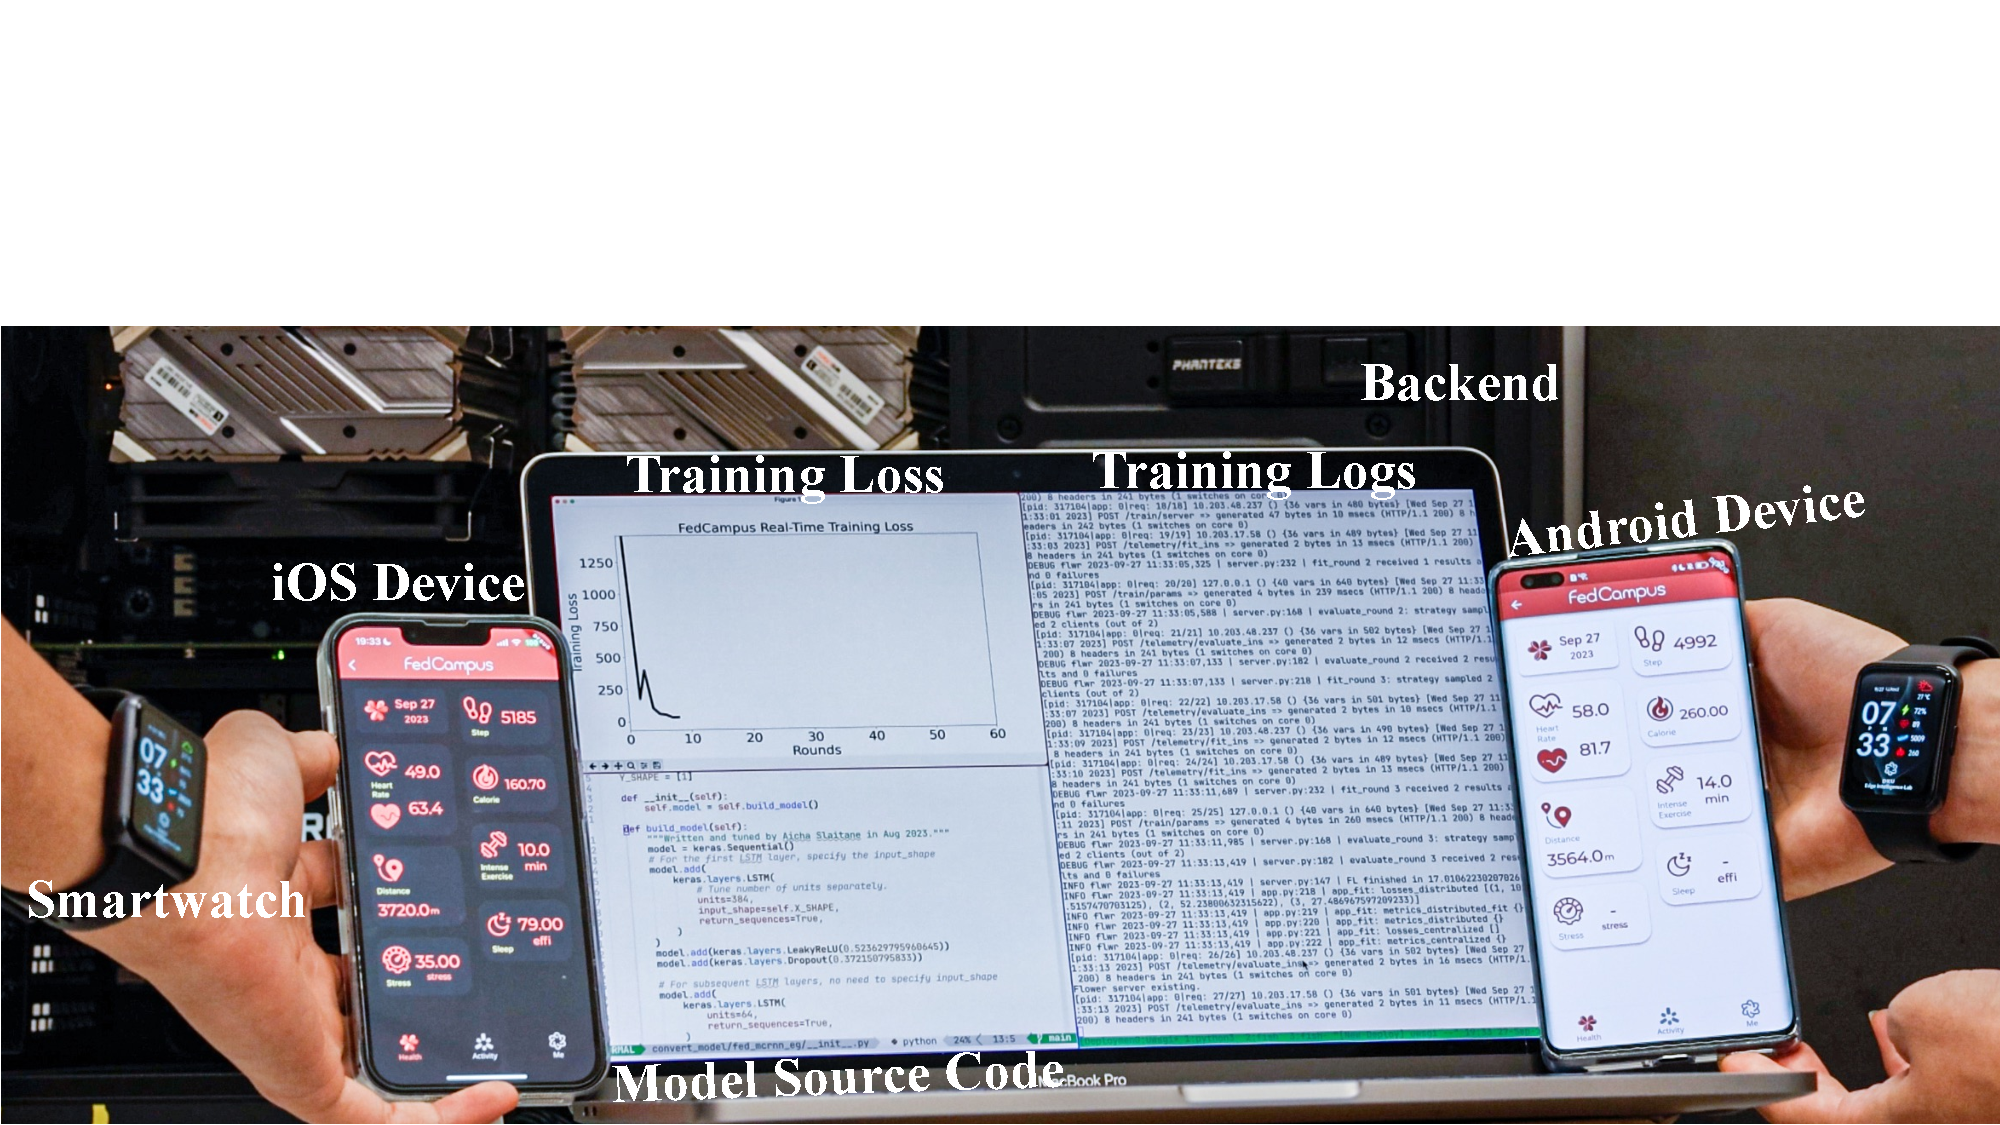
\includegraphics[width=\linewidth]{fedcampus.pdf}
        \caption{Experiment Setup for The \fedkit Integration in The FedCampus
            Application.
        }
    \end{center}\end{figure}

We integrated \fedkit into the \fedcampus Application to
conduct a federated learning experiment using health data on the smartphones,
as displayed in Figure~\ref{fig:integration}.
In our setup,
A backend server is hosted in the physical machine in the background,
while an Android device and an iOS device are running an early version of
the \fedcampus Application.
The laptop is connected to the server via Secure Shell (SSH),
and was displaying the training logs,
along with the training loss and the model's source code.

The \fedcampus Application in this experiment trained a sleep-efficiency
prediction model similar to the model described in~\cite{khoa2022fedmcrnn}
using health data collected from the smartwatches.
Each round of training is instantaneous on both Android because of
the small training dataset,
and both smartphones remained cool with \fedkit's training acceleration.
The models trained on these smartphones are aggregated across Android and iOS,
resulting in a significant reduction in the training loss,
demonstrating \fedkit's effectiveness in real-world scenarios.
